%%%%%%%%%%%%%%%%%%%%%%%%%%%%%%%%%%%%%%%%%%%%%%%%%%%%%%%%%%%%%%%%%%%%%%%%%%%%%%%
%% Plantilla de memoria en LaTeX para la ETSIT - Universidad Rey Juan Carlos
%%
%% Por Gregorio Robles <grex arroba gsyc.urjc.es>
%%     Grupo de Sistemas y Comunicaciones
%%     Escuela Técnica Superior de Ingenieros de Telecomunicación
%%     Universidad Rey Juan Carlos
%% (muchas ideas tomadas de Internet, colegas del GSyC, antiguos alumnos...
%%  etc. Muchas gracias a todos)
%%
%% La última versión de esta plantilla está siempre disponible en:
%%     https://github.com/gregoriorobles/plantilla-memoria
%%
%% Para obtener PDF, ejecuta en la shell:
%%   make
%% (las imágenes deben ir en PNG o JPG)

%%%%%%%%%%%%%%%%%%%%%%%%%%%%%%%%%%%%%%%%%%%%%%%%%%%%%%%%%%%%%%%%%%%%%%%%%%%%%%%%

\documentclass[a4paper, 12pt]{book}
%\usepackage[T1]{fontenc}
%\usepackage[utf8]{inputenc}


%\usepackage[T1]{fontenc} 
%\usepackage[utf8]{inputenc}
%\PrerenderUnicode{ÁáÉéÍíÓóÚúÑñ} % Para que salgan las tildes y demás mierdas en el título.

\usepackage{exmath}


\RequirePackage{MathUnicode} % Paquete para poder poner caracteres griegos y demás cosas raras.
\usepackage[a4paper, left=3.8cm, right=2.5cm, top=3cm, bottom=3cm]{geometry}
\usepackage{times}

%\usepackage[utf8]{inputenc}
\usepackage[spanish]{babel} % Comenta esta línea si tu memoria es en inglés
\usepackage{url}
%\usepackage[dvipdfm]{graphicx}
\usepackage{graphicx}
\usepackage{float}  %% H para posicionar figuras
\usepackage[nottoc, notlot, notlof, notindex]{tocbibind} %% Opciones de índice
\usepackage{latexsym}  %% Logo LaTeX

\usepackage{amsmath} % Matemáticas
\usepackage{amsfonts} % Mas Matemáticas
\usepackage{amssymb} % Mas Matemáticas
\usepackage{amsthm} % Otro paquete de Matemáticas
\usepackage[shadow]{todonotes} % Marcas To Do (a hacer)
\usepackage{xspace} % Espaciado correcto detras de comandos.
\usepackage{mathtools} % Arregla bastantes cosas de los entornos matemáticos por 
\usepackage[acronym]{glossaries} % Glosarios
\usepackage{makeidx}
\usepackage[breaklinks=true]{hyperref}
\usepackage{breakcites}

\interfootnotelinepenalty=10000


\newcommand{\nombreautor}{V\'ictor de Juan Sanz\xspace}
\newcommand{\nombretutor}{Desir\'e Garc\'ia L\'azaro\xspace}
\newcommand{\titulo}{Gamificaci\'on: visión general y aplicación en el aula de Matemáticas\xspace}
\newcommand{\TFM}{Trabajo de Fin de M\'aster\xspace}
\newcommand{\master}{M\'aster en Formaci\'on del Profesorado, especialidad Matem\'aticas\xspace}
%\newcommand{\master}{Máster en Formación del Profesorado: especialidad Matemáticas}

\renewcommand{\rmdefault}{ppl}
\renewcommand{\sfdefault}{fla}
\renewcommand{\ttdefault}{lmtt}
\renewcommand*{\familydefault}{\rmdefault}
\def\@fontsizeopt{11pt}
\message{Loading Palatino fonts}

\newcommand{\coment}[1]{\textit{#1}}

\renewcommand{\baselinestretch}{1.5}  %% Interlineado

\makeglossaries
\newacronym{FPGA}{FPGA}{Field-Programmable Gate Array}

% Glosario

% TODO: Añadir aqu\'i las definiciones del glosario
% Ejemplo de glosario
\newglossaryentry{bitstream}{name={bitstream},description={En este contexto se refiere al binario que configura el Hardware de la FPGA}}



\newacronym{PISA}{PISA}{\textit{Programme for International Student Assessment}}
\newacronym{TIMSS}{TIMSS}{\textit{Trends in International Mathematics and Science Study}}

\newacronym{INEE}{INEE}{Instituto Nacional de Evaluaci\'on Educativa}
\newacronym{INTEF}{INTEF}{Instituto Nacional de Tecnolog\'ias Educativas y Formaci\'on del Profesorado}


\newacronym{PDA}{PDA}{Programaci\'on Did\'actica Anual}


\newacronym{PBL}{PBL}{\textit{Points, Badges and Leaderboards} (Puntos, Medallas y Rankings)}

\newacronym{MUD}{MUD}{\textit{MultiUser Dungeon} -- juegos de rol online}

\newacronym{WCW}{WCW}{\textit{World Gamification Congress} -- Barcelona}

\newglossaryentry{real number}
{
  name={real number},
  description={include both rational numbers, such as $42$ and 
               $\frac{-23}{129}$, and irrational numbers, 
               such as $\pi$ and the square root of two; or,
               a real number can be given by an infinite decimal
               representation, such as $2.4871773339\ldots$ where
               the digits continue in some way; or, the real
               numbers may be thought of as points on an infinitely
               long number line},
  symbol={\ensuremath{\mathbb{R}}}
}

\newacronym{MOOC}{MOOC}{\textit{Massive Online Open Course} -- Curso masivo abierto en l\'inea}

\newacronym{TIC}{TIC}{Tecnolog\'ias de la Informaci\'on y de la Comunicaci\'on}

\makeindex

\newif\iftocs
\tocstrue % Incluye en el índice general: la lista de tablas, lista de figuras y acrónimos.
\tocsfalse % Excluye en el índice general: la lista de tablas, lista de figuras y acrónimos.



\begin{document}
\pagenumbering{Roman} % para empezar la numeración de página con números
\renewcommand{\refname}{Bibliografía}  %% Renombrando
\renewcommand{\appendixname}{Apéndice}

%%%%%%%%%%%%%%%%%%%%%%%%%%%%%%%%%%%%%%%%%%%%%%%%%%%%%%%%%%%%%%%%%%%%%%%%%%%%%%%%
% PORTADA

\begin{titlepage}
\begin{center}
\begin{tabular}[c]{c c}
%\includegraphics[bb=0 0 194 352, scale=0.25]{logo} &
\includegraphics[scale=0.25]{img/logo_vect.png} &
\begin{tabular}[b]{l}
\Huge
\textsf{UNIVERSIDAD} \\
\Huge
\textsf{REY JUAN CARLOS} \\
\end{tabular}
\\
\end{tabular}

\vspace{3cm}

\master

\vspace{0.4cm}

\large
Curso Académico 2016/2017

\vspace{0.8cm}

\TFM

\vspace{2.5cm}

\LARGE
\textsc{\titulo}

\vspace{4cm}

\large
Autor : \nombreautor \\
Tutor : \nombretutor
\end{center}
\end{titlepage}

\newpage
\mbox{}
\thispagestyle{empty} % para que no se numere esta pagina


%%%%%%%%%%%%%%%%%%%%%%%%%%%%%%%%%%%%%%%%%%%%%%%%%%%%%%%%%%%%%%%%%%%%%%%%%%%%%%%%
%%%% Para firmar
\clearpage
%\pagenumbering{gobble}
\chapter*{}
\thispagestyle{empty} % para que no se numere esta pagina

\vspace{-4cm}
\begin{center}
\LARGE
\textbf{\TFM}

\vspace{1cm}
\large
\titulo

\vspace{1cm}
\large
\textbf{Autor :} \nombreautor \\
\textbf{Tutor :} \nombretutor

\end{center}

\vspace{1cm}
La defensa del presente \TFM se realizó el día \qquad$\;\,$ de \qquad\qquad\qquad\qquad \newline de 2017, siendo calificada por el siguiente tribunal:


\vspace{0.5cm}
\textbf{Presidente:}

\vspace{1.2cm}
\textbf{Secretario:}

\vspace{1.2cm}
\textbf{Vocal:}


\vspace{1.2cm}
y habiendo obtenido la siguiente calificación:

\vspace{1cm}
\textbf{Calificación:}


\vspace{1cm}
\begin{flushright}
Fuenlabrada, a \qquad$\;\,$ de \qquad\qquad\qquad\qquad de 2017
\end{flushright}

%%%%%%%%%%%%%%%%%%%%%%%%%%%%%%%%%%%%%%%%%%%%%%%%%%%%%%%%%%%%%%%%%%%%%%%%%%%%%%%%
%%%% Dedicatoria

\chapter*{}
%\pagenumbering{Roman} % para comenzar la numeracion de paginas en numeros romanos
\begin{flushright}
\textit{Dedicado a \\
mi familia / mi abuelo / mi abuela}
\end{flushright}

%%%%%%%%%%%%%%%%%%%%%%%%%%%%%%%%%%%%%%%%%%%%%%%%%%%%%%%%%%%%%%%%%%%%%%%%%%%%%%%%
%%%% Agradecimientos

\chapter*{Agradecimientos}
Aquí vienen los agradecimientos\ldots Aunque está bien acordarse de la pareja,
no hay que olvidarse de dar las gracias a tu madre, que aunque a veces no lo 
parezca disfrutará tanto de tus logros como tú\ldots Además, la pareja quizás
no sea para siempre, pero tu madre sí.



%%%%%%%%%%%%%%%%%%%%%%%%%%%%%%%%%%%%%%%%%%%%%%%%%%%%%%%%%%%%%%%%%%%%%%%%%%%%%%%%
%%%% Resumen

\chapter*{Resumen}
%\addcontentsline{toc}{chapter}{Resumen} % si queremos que aparezca en el ?dice
\markboth{RESUMEN}{RESUMEN} % encabezado

Incluir un texto de máximo 15 líneas en el que cuentes todo lo que has hecho en tu  tfm, debajo como máximo 5 palabras claves, y exactamente lo mismo traducido al ingles, abstract y key words.


%%%%%%%%%%%%%%%%%%%%%%%%%%%%%%%%%%%%%%%%%%%%%%%%%%%%%%%%%%%%%%%%%%%%%%%%%%%%%%%%
%%%% Resumen en inglés

\chapter*{Summary}
%!TEX root = ../TFM.tex
%\addcontentsline{toc}{chapter}{Resumen} % si queremos que aparezca en el ?dice
\markboth{RESUMEN}{RESUMEN} % encabezado


Innovation and improvement are necessary in the Spanish education environment.
%
The last education law approved, Ley Orgánica para la Mejora de la Calidad Educativa, has it included in its name.

Eventhough there are not enough, there are increasingly more teachers and institutions including the new advances to their praxis inside the classrooms.
%
It is important to support these initiatives and provide them with resources and possibilities.  
%
This paper tries precisely to do so, offer a detailed study of Gamification as a strategy for the classroom followed by a concrete proposal, designed and detailed, ready to be implemented inside the classroom.


\begin{keywordsEn}
Gamification, Players Taxonomy, Motivation and Flow theories, PISA Reports , Didactic Unit, Mathematics, High School, LOMCE
\end{keywordsEn}

\cleardoublepage

%%%%%%%%%%%%%%%%%%%%%%%%%%%%%%%%%%%%%%%%%%%%%%%%%%%%%%%%%%%%%%%%%%%%%%%%%%%%%%%%
%%%%%%%%%%%%%%%%%%%%%%%%%%%%%%%%%%%%%%%%%%%%%%%%%%%%%%%%%%%%%%%%%%%%%%%%%%%%%%%%
% ÍNDICES %
%%%%%%%%%%%%%%%%%%%%%%%%%%%%%%%%%%%%%%%%%%%%%%%%%%%%%%%%%%%%%%%%%%%%%%%%%%%%%%%%

% Las buenas noticias es que los índices se generan automáticamente.
% Lo único que tienes que hacer es elegir cuáles quieren que se generen,
% y comentar/descomentar esa instrucción de LaTeX.
%%%% Índice de figuras


%%%% Índice de contenidos
\tableofcontents 


%%%% Índice de figuras
\cleardoublepage

\iftocs
\addcontentsline{toc}{chapter}{Lista de figuras.}% para que aparezca en el indice de contenidos
\else
\fi

\listoffigures % indice de figuras



%%%% Índice de tablas
\cleardoublepage

\iftocs
\addcontentsline{toc}{chapter}{Lista de tablas}% para que aparezca en el indice de contenidos
\else
\fi
\listoftables % indice de tablas

\iftocs
\addcontentsline{toc}{chapter}{Acrónimos}% para que aparezca en el indice de contenidos
\else
\fi

 
\printglossary[title=Glosario,toctitle=Glosario]
\printglossary[title=Acrónimos,toctitle=Acrónimos,type=\acronymtype]


%%%%%%%%%%%%%%%%%%%%%%%%%%%%%%%%%%%%%%%%%%%%%%%%%%%%%%%%%%%%%%%%%%%%%%%%%%%%%%%%
%%%%%%%%%%%%%%%%%%%%%%%%%%%%%%%%%%%%%%%%%%%%%%%%%%%%%%%%%%%%%%%%%%%%%%%%%%%%%%%%
% INTRODUCCIÓN %
%%%%%%%%%%%%%%%%%%%%%%%%%%%%%%%%%%%%%%%%%%%%%%%%%%%%%%%%%%%%%%%%%%%%%%%%%%%%%%%%

\cleardoublepage
\pagenumbering{arabic} % para empezar la numeración de página con números
\chapter{Introducción}
\label{chap:intro} % etiqueta para poder referenciar luego en el texto con ~\ref{sec:intro}


\section{Estado actual de la Educación de Matemáticas en España}
\label{sec:EstadoEducacionMates}

En esta sección se introducirá al lector en la situación actual de la enseñanza de Matemáticas en España. 
%
Se tratarán 2 temas fundamentales: la comparativa de España con otros países en la enseñanza de Matemáticas y las actitudes y problemas concretos de la educación de Matemáticas en España.


\paragraph{Informes Internacionales (en Matemáticas)} 

Fundamentalmente utilizaremos los informes \gls{PISA} \cite{InformePisa2012}, \cite{InformePisa2015}, centrándonos exclusivamente en Matemáticas.

En \cite{InformePisa2012} España se sitúa en la posición 33 (de 65) con una puntuación de 484 puntos, siendo esta puntuación inferior a la media OCDE de ese año (494) y a la media UE (489).
%
En el siguiente informe PISA \cite{InformePisa2015}, se produce una mejora en España. 
%
La puntuación es mayor siendo la tendencia internacional negativa. 
%
Sin embargo, la puntuación española sigue por debajo de la media.
%
En la tabla \ref{tbl::ResumenPisa} se encuentran agrupados estos datos.

\begin{table}[hbtp]
\centering
\begin{tabular}{ccccc}
Año & Posición España & Puntuación España & Media OCDE & Media UE\\\hline
2012 & 33 & 484 & 494 & 489\\
2015 & 29 & 486 & 490 & 493
\end{tabular}
\caption{Resumen resultados Pisa}
\label{tbl::ResumenPisa}
\end{table}

No obstante, es necesario mencionar que no todas las comunidades autónomas obtienen los mismos resultados. 
%
Por ejemplo, en 2015, algunas comunidades autónomas como Navarra (518), Castilla y León (506), La Rioja (505) y la Comunidad de Madrid (503) se sitúan por encima de la media OCDE.


Otra información relevante aportada por los informes PISA es el porcentaje de estudiantes excelentes (nivel 5 ó 6 de las pruebas) y el porcentaje de estudiantes rezagados (nivel 1 o inferior).
%
En la figura \ref{fig::PisaRezEx} se encuentran las gráficas de las tendencias obtenidas en España y en la OCDE según los informes PISA desde 2002.


\begin{figure}[hbtp]
\centering
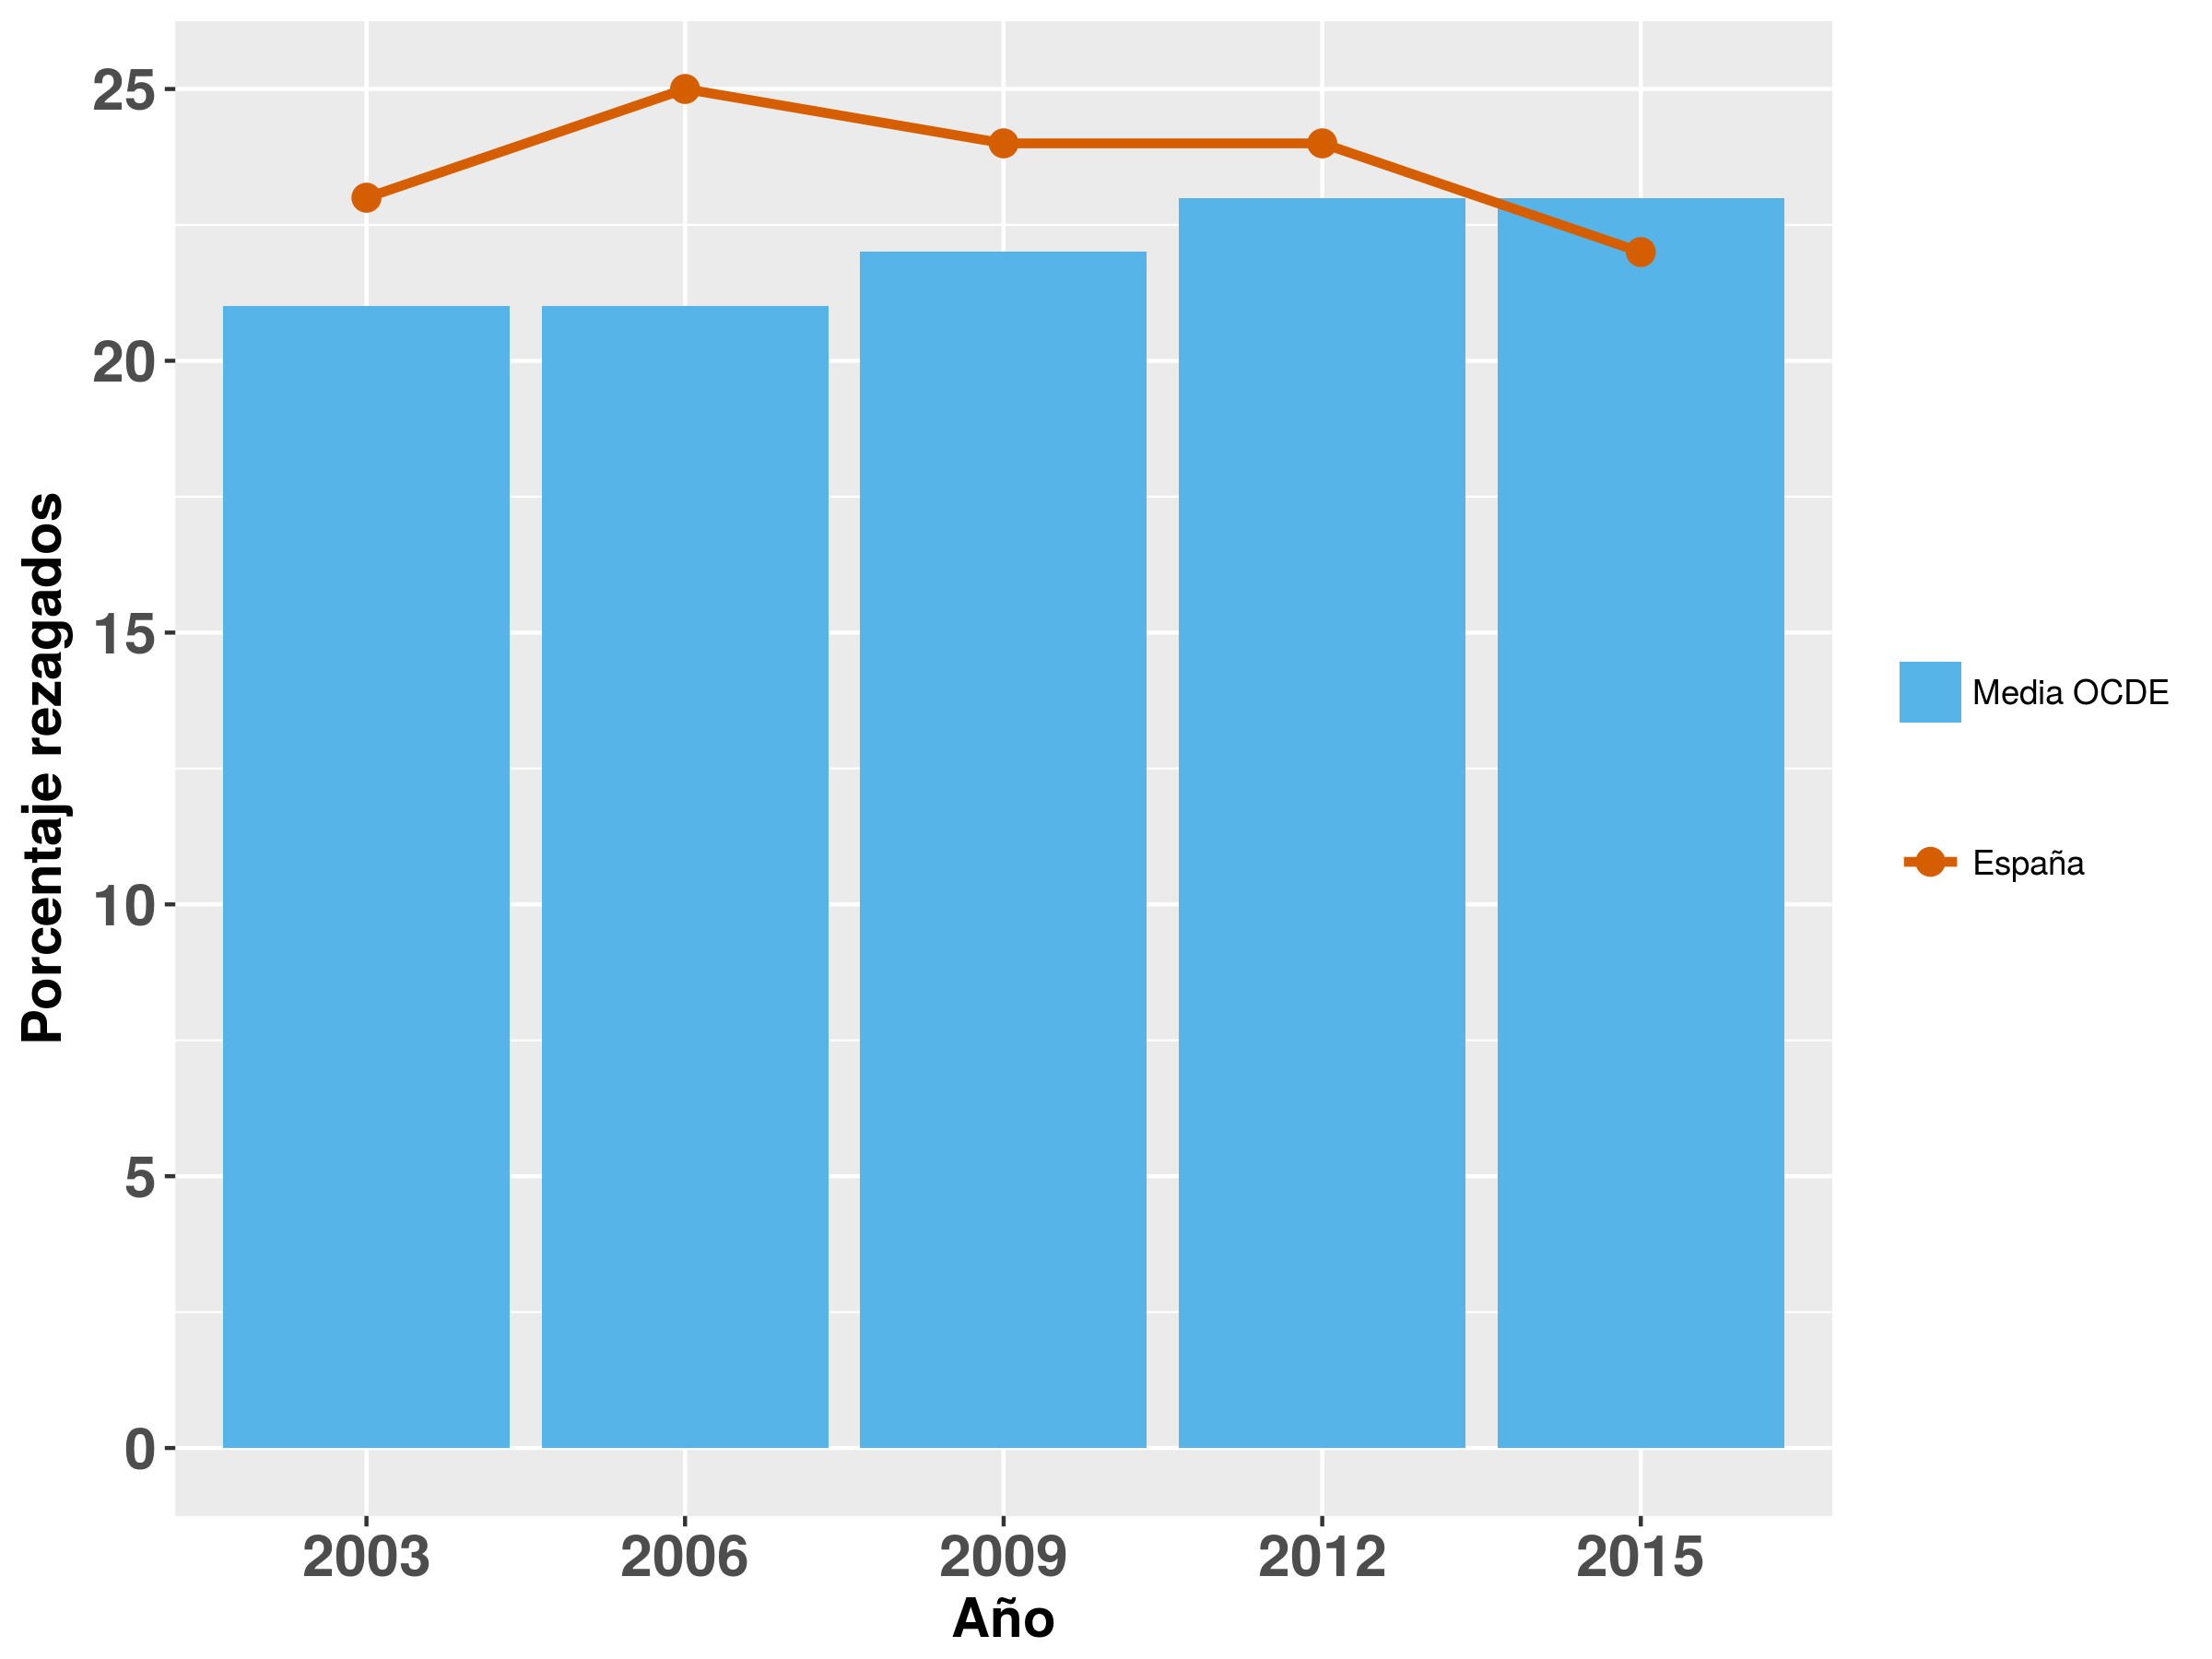
\includegraphics[scale=0.62]{img/PisaRezagados.png}
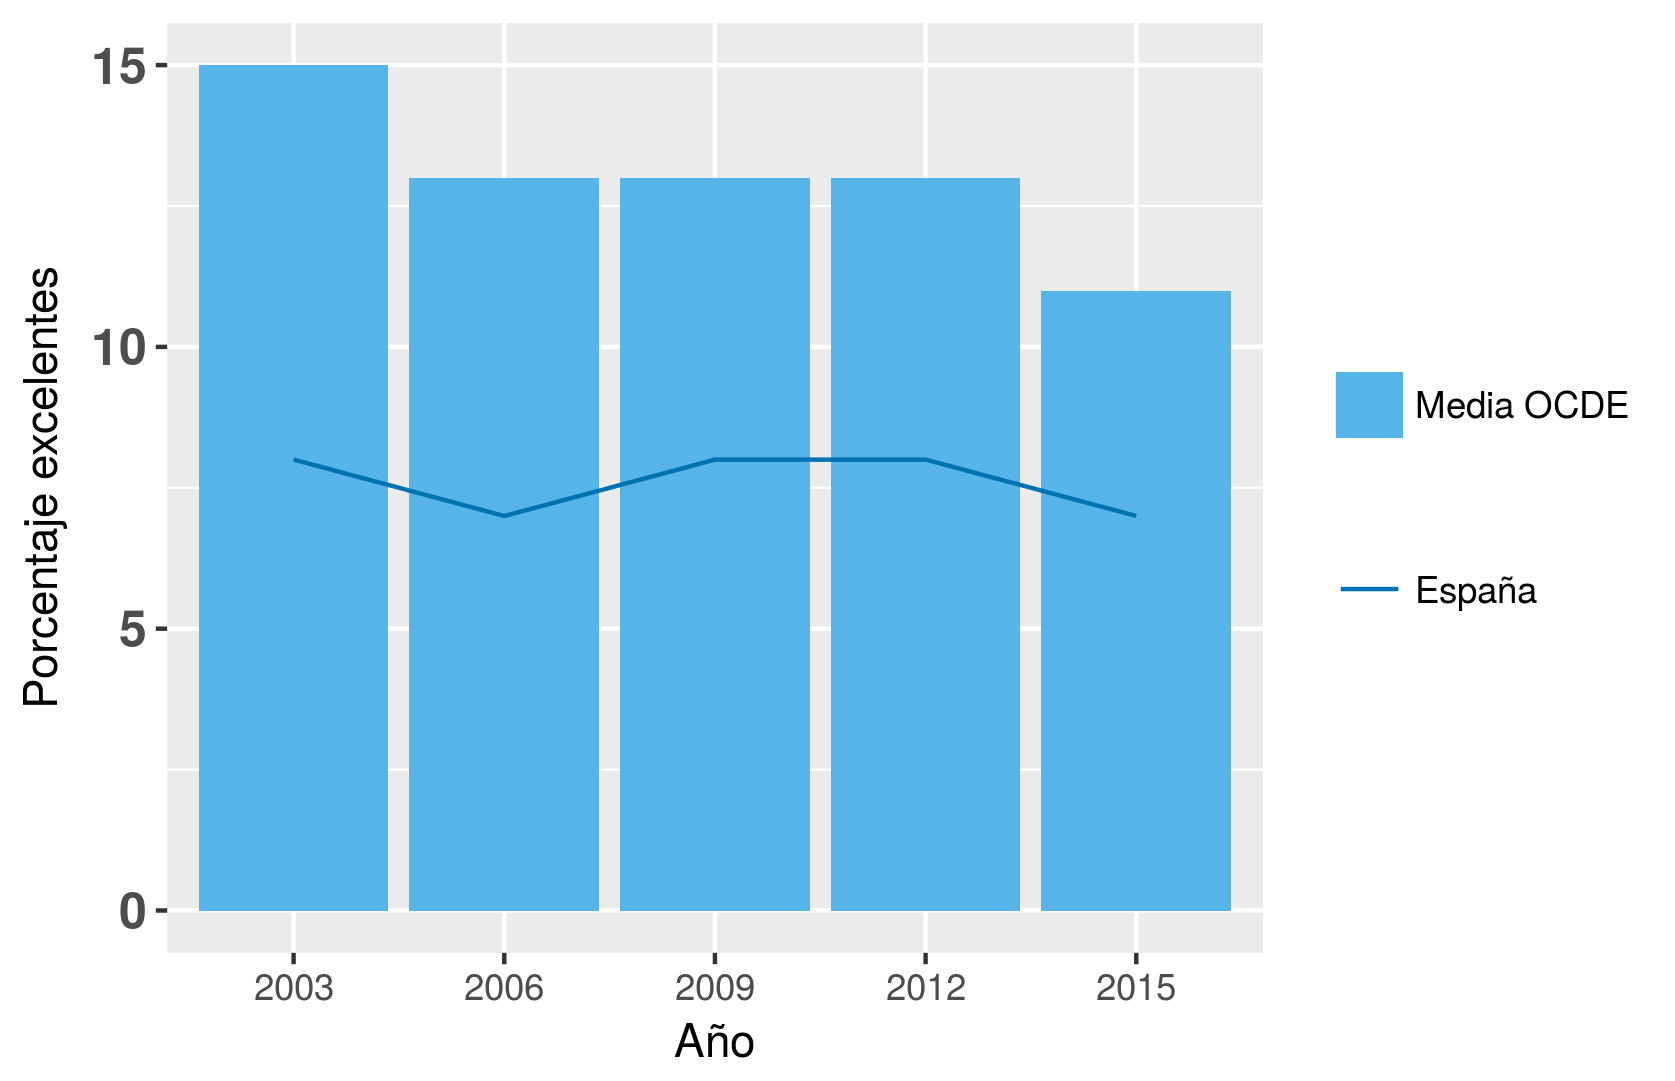
\includegraphics[scale=0.62]{img/PisaExcelentes.png}
\caption{Comparativa de estudiantes rezagados (imagen superior) y excelentes (imagen inferior) en España y en los países OCDE. \newline{} Fuente: Elaboración propia a partir de los informes PISA.}
\label{fig::PisaRezEx}
\end{figure}


En el porcentaje de estudiantes rezagados se puede apreciar una ligera mejora en la tendencia española frente a un empeoramiento de la tendencia internacional.
%
A pesar de ello, casi uno de cada 4 adolescentes posee un nivel 1 o inferior de habilidad matemática. 
%
Esta situación es claramente mejorable.
%
Por otro lado, el porcentaje de estudiantes excelentes en España se mantiene estable en torno al 7\% u 8\% (dependiendo del año), siendo inferior a la media internacional.


Debido a que el informe PISA es un informe descriptivo, vamos a recurrir a \cite{ActitudesHaciaMates} para descubrir algunos aspectos influyentes en la educación matemática en España.


\paragraph{Estudio Nacional}

En el trabajo \cite{ActitudesHaciaMates} se realiza un estudio transversal para explorar las actitudes hacia las Matemáticas de alumnos en el sistema educativo español, desde tercero de E.P. hasta el primer curso universitario. 
%
Se centra sobretodo en explicar el rechazo de los estudiantes hacia las Matemáticas.
%
El estudio apoya la existencia de un círculo vicioso: dificultad $\to$ aburrimiento$\to$ suspenso$\to$ fatalismo$\to$ bajo autoconcepto$\to$ desmotivación$\to$ rechazo$\to$ dificultad.
\label{circuloVicioso}


%El modelo construido utiliza 7 variables (de las 40 estudiadas) que presentamos a continuación, ordenadas según su influencia: \begin{itemize}
%\vspace{-0.4cm}\item Percepción de materia aburrida-divertida.
%\vspace{-0.4cm}\item Percepción de materia fácil-difícil.
%\vspace{-0.4cm}\item Percepción de competencias para las Matemáticas.
%\vspace{-0.4cm}\item Influencia del profesor sobre el rechazo (El rechazo hacia las Matemáticas se debe, en cierta medida, a los profesores de Matemáticas que el estudiante ha tenido). La relación es lineal: valores altos de rechazo se correlacionan con valores altos de influencia, mientras que valores bajos de rechazo se correlacionan con valores bajos de influencia.
%\vspace{-0.4cm}\item Atribución de causalidad de éxito en Matemáticas: los estudiantes consideran que las aptitudes ejercen una mayor influencia en el desempeño que la dedicación y el estudio.
%\vspace{-0.4cm}\item Competencia percibida para el cálculo mental.
%\vspace{-0.4cm}\item Dificultad percibida para el aprendizaje matemático.
%\end{itemize}

Al trabajar con una muestra representativa de diversas edades, se puede valorar la influencia de la edad en el rechazo hacia las Matemáticas, comprobándose que el rechazo hacia las Matemáticas aumenta con la edad y las relaciones predictivas se hacen más fuertes.
%
Por ejemplo, el porcentaje de alumnos que rechazan las Matemáticas en 3 de E.P. es del 13.10\%, en 5 E.P. del 28\%  y el de estudiantes de 3 E.S.O. es del 49.50\%.
%
Parece que es en la E.S.O. donde se produce un gran aumento del rechazo hacia las Matemáticas.


\cite{ActitudesHaciaMates} establece que la variable más importante\footnote{Al menos de las 40 estudiadas}. es la percepción de la materia en la escala aburrida-divertida, seguida por la percepción de dificultad.


\paragraph{Conclusión:} El presente trabajo pretende ofrecer una respuesta a la situación de las Matemáticas actuales.
%
Ofrecemos una propuesta metodológica para romper el círculo vicioso (ver \ref{circuloVicioso}) en los eslabones de la desmotivación y el aburrimiento.

Por otro lado, creemos que esta propuesta metodológica tiene mucho potencial en Educación Secundaria, ya que es donde se produce el aumento brusco del rechazo.
%
Si en los cursos de la E.S.O. se consiguiera influir en las percepciones de los estudiantes aparejando Matemáticas con diversión se podrían reducir drásticamente el porcentaje de alumnos rezagados en Matemáticas (ver \ref{fig::PisaRezEx}) y mejorar el nivel matemático general.


\section{La Gamificación}

\coment{Esto es lo que correspondería al marco teórico.}

En esta sección procedemos a describir a nivel general la Gamificación. 
%
La Gamificación entendida como una técnica que puede ser aplicada a muchos ámbitos, no sólo al educativo. 
%
Primeramente trataremos de clarificar el concepto de gamificación, porqué y cómo se puede gamificar un contexto.
%
Una vez detallado, en la siguiente sección trataremos de aplicar la gamificación al aula.



\coment{Qué es la Gamificación}

Gamificación o ludificación, optamos por Gamificación porque...

Atendiendo a \cite{GamificationDef} podemos definir \concept{Gamificación} como \textit{el uso de elementos de juegos en contextos no lúdicos}. 

Algunos de los elementos que hacen atractivos los juegos son
\textbf{Feedback instantáneo}
poder tomar \textbf{decisiones importantes},
\textbf{bucles de atracción y de fracaso},
\textbf{niveles de dificultad progresiva}... La idea es incorporar esos elementos en algún contexto no lúdico (en general, no sólo en la educación\footnote{No querría centrarme sólo en la educación para dar una visión más general de la gamificación como técnica en muchos campos: marketing, negocios... Creo que ofrece un punto de vista más riguroso y científico hablar de Gamificación en general y no sólo Gamificación en la educación.}).


\coment{Por qué gamificar}

Alguna lectura sobre porqué gamificar conceptualmente.

Porque funciona. Conclusiones de \cite{EmpiricalGamification}


\subsection{Diferencias entre Juegos serios y Gamificación}

Son conceptos distintos. Los \concept[Juegos serios]{juegos serios} son \cite{GamificationDef}... mientras que la gamificación consiste en...

Aunque los juegos serios pueden ser interesantes (conclusiones de \cite{MetaSerious}), se salen de este estudio.


\subsection{Elementos de la Gamificación}

\paragraph{Pensando como un diseñador}
\paragraph{La anatomía de la diversión}

Los elementos de la Gamificación son los elementos que podemos encontrar en los juegos, atendiendo a \cite{Hunicke04mda:a} son dinámicas, mecánicas y componentes.


\subsubsection{Dinámicas}

\subsubsection{Mecánicas}

\subsubsection{Componentes}



\paragraph{Puntos ...} \gls{pbl}

\subparagraph*{Puntos}

\subparagraph*{Medallas}

\subparagraph*{Leaderboards}

Los leaderboards desmotivan al 80\% de la gente. 

Podríamos definir competición utilizando la definición de \cite{Crawford_CompetitionDef} Competition is when students are “constrained from impeding each other and instead devote the entirety of their attentions to optimizing their own performance.”

Crean una competición con la que hay que tener cuidado. Leyendo \cite{CompetitionInEd}...

\subsubsection{Impacto de la motivación}

\paragraph{Posibles peligros}

Ya hemos constatado un posible peligro al describir el componente \textit{leaderboard}. Además, hay otros.

Más competidores, menos motivación. \cite{n-effect}

Premios para los ganadores deberían ser de poca importancia o incluso simbólicos para asegurar que el esfuerzo de los estudiantes es intrínseco y no está dirigido por la expetativa del premio \cite{CompetitionInEd}.

\section{Educación gamificada}

Hasta ahora hemos hablado en términos generales de la gamificación. 
%
En esta sección trataremos de estudiar cómo se adapta esa teoría general al ecosistema de un aula.

\cite{lee2011gamification} constata varias cosas.

Hay otros estudios interesantes como \cite{Hanus2015152} y \cite{ReviewGamificationInEducation}.

\subsection{Potencial de la gamificación en el aula}

En la sección \ref{sec:EstadoEducacionMates} hemos constatado algunos problemas. 
%
Vamos a ir viendo cómo la Gamificación puede atajar esos problemas concretos y también, qué problemas se quedarían sin atajar.

\subsubsection{¿Es una metodología inclusiva?}

Esta pregunta es importante, pero no hay que descartar la metodología en caso de que la respuesta sea negativa, ya que también es importante plantearse:  ¿Es una metodología \textbf{más inclusiva} que la tradicional?
%
Tal vez no es una metodología perfecta, pero sí una metodología que aporta mejoras.



%%%%%%%%%%%%%%%%%%%%%%%%%%%%%%%%%%%%%%%%%%%%%%%%%%%%%%%%%%%%%%%%%%%%%%%%%%%%%%%%
%%%%%%%%%%%%%%%%%%%%%%%%%%%%%%%%%%%%%%%%%%%%%%%%%%%%%%%%%%%%%%%%%%%%%%%%%%%%%%%%
% DISEÑO E IMPLEMENTACIÓN %
%%%%%%%%%%%%%%%%%%%%%%%%%%%%%%%%%%%%%%%%%%%%%%%%%%%%%%%%%%%%%%%%%%%%%%%%%%%%%%%%

\cleardoublepage
\chapter{Gamificar las Matemáticas}

\section{¿Se pueden gamificar las Matemáticas?}

Lo siguiente que necesitamos, si estamos convencidos de que la Gamificación puede ser una buena metodología, es tratar cómo se puede gamificar un aula.
%
Dedicaremos el próximo capítulo a ello.

\section{Estado de la Ley y del currículo}

Primero: ¿Permite o incluso anima la ley al empleo de esta metodología?

Segundo: Necesitamos elegir un curso y su currículo.

\subsection{Elección del curso para Gamificar}

El curso elegido es: porque...

\subsubsection{Contenidos de ese curso}
\subsubsection{Estándares de Aprendizaje Evaluables}


\section{Elementos de la gamificación aplicables al aula de Matemáticas}

\paragraph{Dinámicas}

\subparagraph{Narrativa}
\subparagraph{Progresión}

\paragraph{Mecánicas}

Las mecánicas que utilizaremos serán:
\subparagraph{Retos},
\subparagraph{Competición y cooperación},
\subparagraph{Feedback},
\subparagraph{Premios}

 Los premios serán: logros, medallas, puntos (que describiremos a continuación).

\paragraph{Elementos}

Los elementos que utilizaremos serán:
\subparagraph{Niveles},
\subparagraph{Logros},
\subparagraph{Puntos},
\subparagraph{Medallas},
\subparagraph{Jefes finales}...

\section{Programación anual Gamificada}

\subsection{Aprendizaje competencial}
\subsection{Cobertura de los contenidos}
\subsection{Incorporación de los Estándares de Aprendizaje Evaluables}

Matriz de trazabilidad entre los Estándares de Aprendizaje Evaluables y los componentes de la Gamificación:
\begin{table}[hbtp]
\begin{tabular}{c|c}
& Estándares de Aprendizaje Evaluables\\\hline
Elementos & \\\hline
\end{tabular}
\label{Trazabilidad}
\caption{Matriz de trazabilidad entre los Estándares de Aprendizaje Evaluables y los componentes de la Gamificación.}
\end{table}


\section{Evaluación de la gamificación}

Es fundamental saber si la gamificación tal como se ha llevado a cabo ha merecido la pena, qué aspectos son mejorables y cuáles hay que mantener.
%
Podríamos utilizar el marco propuesto por \cite{EvaluacionGamificacion} para autoevaluar la gamificación realizada.


%%%%%%%%%%%%%%%%%%%%%%%%%%%%%%%%%%%%%%%%%%%%%%%%%%%%%%%%%%%%%%%%%%%%%%%%%%%%%%%%
%%%%%%%%%%%%%%%%%%%%%%%%%%%%%%%%%%%%%%%%%%%%%%%%%%%%%%%%%%%%%%%%%%%%%%%%%%%%%%%%
% CONCLUSIONES %
%%%%%%%%%%%%%%%%%%%%%%%%%%%%%%%%%%%%%%%%%%%%%%%%%%%%%%%%%%%%%%%%%%%%%%%%%%%%%%%%

\cleardoublepage
\chapter{Conclusiones}
\label{chap:conclusiones}


%Se comenta pero no se pone como apartado específico: 
% \section{Trabajos futuros}

\label{sec:trabajos_futuros}

Puesta en marcha y evaluación. Detectar posibles mejoras.

Propuestas de Gamificación para otros cursos y otras asignaturas.



%%%%%%%%%%%%%%%%%%%%%%%%%%%%%%%%%%%%%%%%%%%%%%%%%%%%%%%%%%%%%%%%%%%%%%%%%%%%%%%%
%%%%%%%%%%%%%%%%%%%%%%%%%%%%%%%%%%%%%%%%%%%%%%%%%%%%%%%%%%%%%%%%%%%%%%%%%%%%%%%%
% APÉNDICE(S) %
%%%%%%%%%%%%%%%%%%%%%%%%%%%%%%%%%%%%%%%%%%%%%%%%%%%%%%%%%%%%%%%%%%%%%%%%%%%%%%%%

\cleardoublepage
\appendix


%%%%%%%%%%%%%%%%%%%%%%%%%%%%%%%%%%%%%%%%%%%%%%%%%%%%%%%%%%%%%%%%%%%%%%%%%%%%%%%%
%%%%%%%%%%%%%%%%%%%%%%%%%%%%%%%%%%%%%%%%%%%%%%%%%%%%%%%%%%%%%%%%%%%%%%%%%%%%%%%%
% BIBLIOGRAFIA %
%%%%%%%%%%%%%%%%%%%%%%%%%%%%%%%%%%%%%%%%%%%%%%%%%%%%%%%%%%%%%%%%%%%%%%%%%%%%%%%%

\cleardoublepage

% Las siguientes dos instrucciones es todo lo que necesitas
% para incluir las citas en la memoria
\bibliographystyle{apalike}
\bibliography{memoria}  % memoria.bib es el nombre del fichero que contiene
% las referencias bibliográficas. Abre ese fichero y mira el formato que tiene,
% que se conoce como BibTeX. Hay muchos sitios que exportan referencias en
% formato BibTeX. Prueba a buscar en http://scholar.google.com por referencias
% y verás que lo puedes hacer de manera sencilla.
% Más información: 
% http://texblog.org/2014/04/22/using-google-scholar-to-download-bibtex-citations/

\printindex

\end{document}
